\documentclass[12pt,a4paper]{article}

% ---- Codificacao e fontes ----
\usepackage[utf8]{inputenc}
\usepackage[T1]{fontenc}
\usepackage{mathptmx} % Times New Roman

% ---- Layout ABNT ----
\usepackage[left=3cm,top=3cm,right=2cm,bottom=2cm]{geometry}
\usepackage{setspace}
\usepackage{indentfirst}
\usepackage{graphicx}
\usepackage{titlesec}
\usepackage{fancyhdr}
\usepackage{enumitem}
\usepackage{hyperref}
\hypersetup{hidelinks}

% Rotulos em portugues (sem babel)
\renewcommand{\contentsname}{SUMÁRIO}
\renewcommand{\refname}{REFERÊNCIAS}
\renewcommand{\figurename}{Figura}
\setlength{\emergencystretch}{3em}

% Recuo de paragrafo ABNT (1,25 cm) e espacamento 1,5
\setlength{\parindent}{1.25cm}
\onehalfspacing

% Titulos de secao em negrito, caixa alta nas secoes primarias
\titleformat{\section}{\normalfont\bfseries}{\thesection}{1em}{\MakeUppercase}
\titleformat{\subsection}{\normalfont\bfseries}{\thesubsection}{1em}{}
\titlespacing*{\section}{0pt}{12pt}{6pt}
\titlespacing*{\subsection}{0pt}{10pt}{4pt}

% Numero de pagina no canto superior direito
\pagestyle{fancy}
\fancyhf{}
\renewcommand{\headrulewidth}{0pt}
\fancyhead[R]{\thepage}

\begin{document}

% ================= CAPA =================
\begin{titlepage}
\thispagestyle{empty}
\begin{center}
{\bfseries FACULDADE DE INFORMÁTICA E ADMINISTRAÇÃO PAULISTA -- FIAP}

\vspace{3cm}

LINCOLN SIMÃO PEREIRA -- RM567284\\
MIGUEL SILVA BEZERRA -- RM566763\\
NICOLAS SAKAUE NISHIMURA -- RM567752

\vspace{3.5cm}

{\bfseries\large GLOBAL SOLUTION 2\textordmasculine/2026 -- POO\\[0.3cm]
SENTINELA DO TERRITÓRIO: MONITORAMENTO DE RISCO DE ALAGAMENTO (CITIZENTECH)}

\vfill

São Paulo\\
2026
\end{center}
\end{titlepage}

% ================= FOLHA DE ROSTO =================
\newpage
\thispagestyle{empty}
\begin{center}
LINCOLN SIMÃO PEREIRA -- RM567284\\
MIGUEL SILVA BEZERRA -- RM566763\\
NICOLAS SAKAUE NISHIMURA -- RM567752

\vspace{4cm}

{\bfseries\large SENTINELA DO TERRITÓRIO: MONITORAMENTO DE RISCO DE ALAGAMENTO (CITIZENTECH)}
\end{center}

\vspace{2cm}

\begin{flushright}
\begin{minipage}{0.55\textwidth}
\onehalfspacing\small
Documento da disciplina de \textit{Object-Oriented Programming}, apresentado à FIAP como requisito parcial para avaliação da Global Solution do 2\textordmasculine\ semestre de 2026, sob orientação do Prof. Ygor Moraes Martins dos Anjos.
\end{minipage}
\end{flushright}

\vfill
\begin{center}
São Paulo\\
2026
\end{center}

% ================= SUMARIO =================
\newpage
\tableofcontents
\thispagestyle{empty}

% ================= TEXTO =================
\newpage

\section{Introdução}

O tema CitizenTech propõe o uso da tecnologia para atender necessidades reais das pessoas nas cidades e comunidades. Dentro desse contexto, este trabalho apresenta o \textit{Sentinela do Território}, uma plataforma de monitoramento territorial desenvolvida com os conceitos de Programação Orientada a Objetos (POO).

O recorte escolhido foi o \textbf{clima local}, com foco em chuva intensa e risco de alagamento em pontos vulneráveis. O sistema lê medições de sensores, calcula previsões simples sobre o nível do rio e emite alertas automáticos classificados por severidade, respondendo à pergunta central da proposta: qual problema vai atingir o território nos próximos períodos e o que se pode fazer hoje para reduzir o impacto.

\section{Objetivos}

O objetivo geral é construir um protótipo em console que demonstre, na prática, os pilares da POO aplicados a um problema real de defesa civil. São objetivos específicos: (i) modelar os componentes do território e os dispositivos de monitoramento; (ii) proteger os dados sensíveis da comunidade por meio de encapsulamento; (iii) oferecer diferentes estratégias de previsão por meio de herança e polimorfismo; e (iv) emitir alertas que expliquem o seu motivo, apoiando — e não substituindo — a decisão humana.

\section{Fundamentação: conceitos de POO aplicados}

\subsection{Classe abstrata}
A classe \texttt{ComponenteTerritorial} é abstrata: não pode ser instanciada, pois não existe um componente genérico no território. Ela reúne atributos comuns (identificador, nome, região e status) e comportamentos concretos (ativar e desativar), além de declarar o método abstrato \texttt{verificarStatus()}, que cada subclasse implementa à sua maneira.

\subsection{Interface}
A interface \texttt{Sensor} define o contrato que todo sensor deve cumprir: ler valor, verificar funcionamento, informar tipo e unidade e detectar quando a leitura ultrapassa o limite. Três sensores implementam o contrato — \texttt{SensorChuva}, \texttt{SensorNivelRio} e \texttt{SensorUmidade} — garantindo uma interface comum, independentemente da implementação interna de cada um.

\subsection{Encapsulamento}
A classe \texttt{DadosTerritorio} mantém todos os atributos privados. Os limiares de alerta, que disparam ações de emergência, são informações sensíveis e só podem ser alterados mediante um código de acesso. Toda alteração é validada: população negativa e limiares fora de faixa (que não respeitem a ordem atenção $<$ alerta $<$ crítico) são rejeitados com mensagem clara, preservando o último valor válido.

\subsection{Herança e polimorfismo}
A classe abstrata \texttt{EstrategiaPrevisao} define o que é comum a toda previsão. Dela herdam \texttt{PrevisaoMediaMovel} (média das últimas N leituras) e \texttt{PrevisaoComparacao} (compara o período atual com o anterior e projeta a tendência). Cada subclasse possui atributos próprios, usa \texttt{super()} para reaproveitar a classe mãe e sobrescreve o método \texttt{prever()}, de modo que o mesmo comando produz comportamentos diferentes conforme a estratégia.

\section{Desenvolvimento}

\subsection{Arquitetura das classes}
O sistema é composto por doze classes. Além das citadas, \texttt{EstacaoDeColeta} e \texttt{PainelInformativo} herdam de \texttt{ComponenteTerritorial}; a estação, em particular, \textit{tem} sensores a bordo (associação), reunindo as leituras do território. A classe \texttt{SistemaMonitoramento} concentra o menu interativo e o motor de alertas. A Figura~\ref{fig:classes} apresenta o diagrama de classes completo, com as três hierarquias e as associações.

\begin{figure}[h]
\centering
\caption{Diagrama de classes do Sentinela do Território.}
\label{fig:classes}
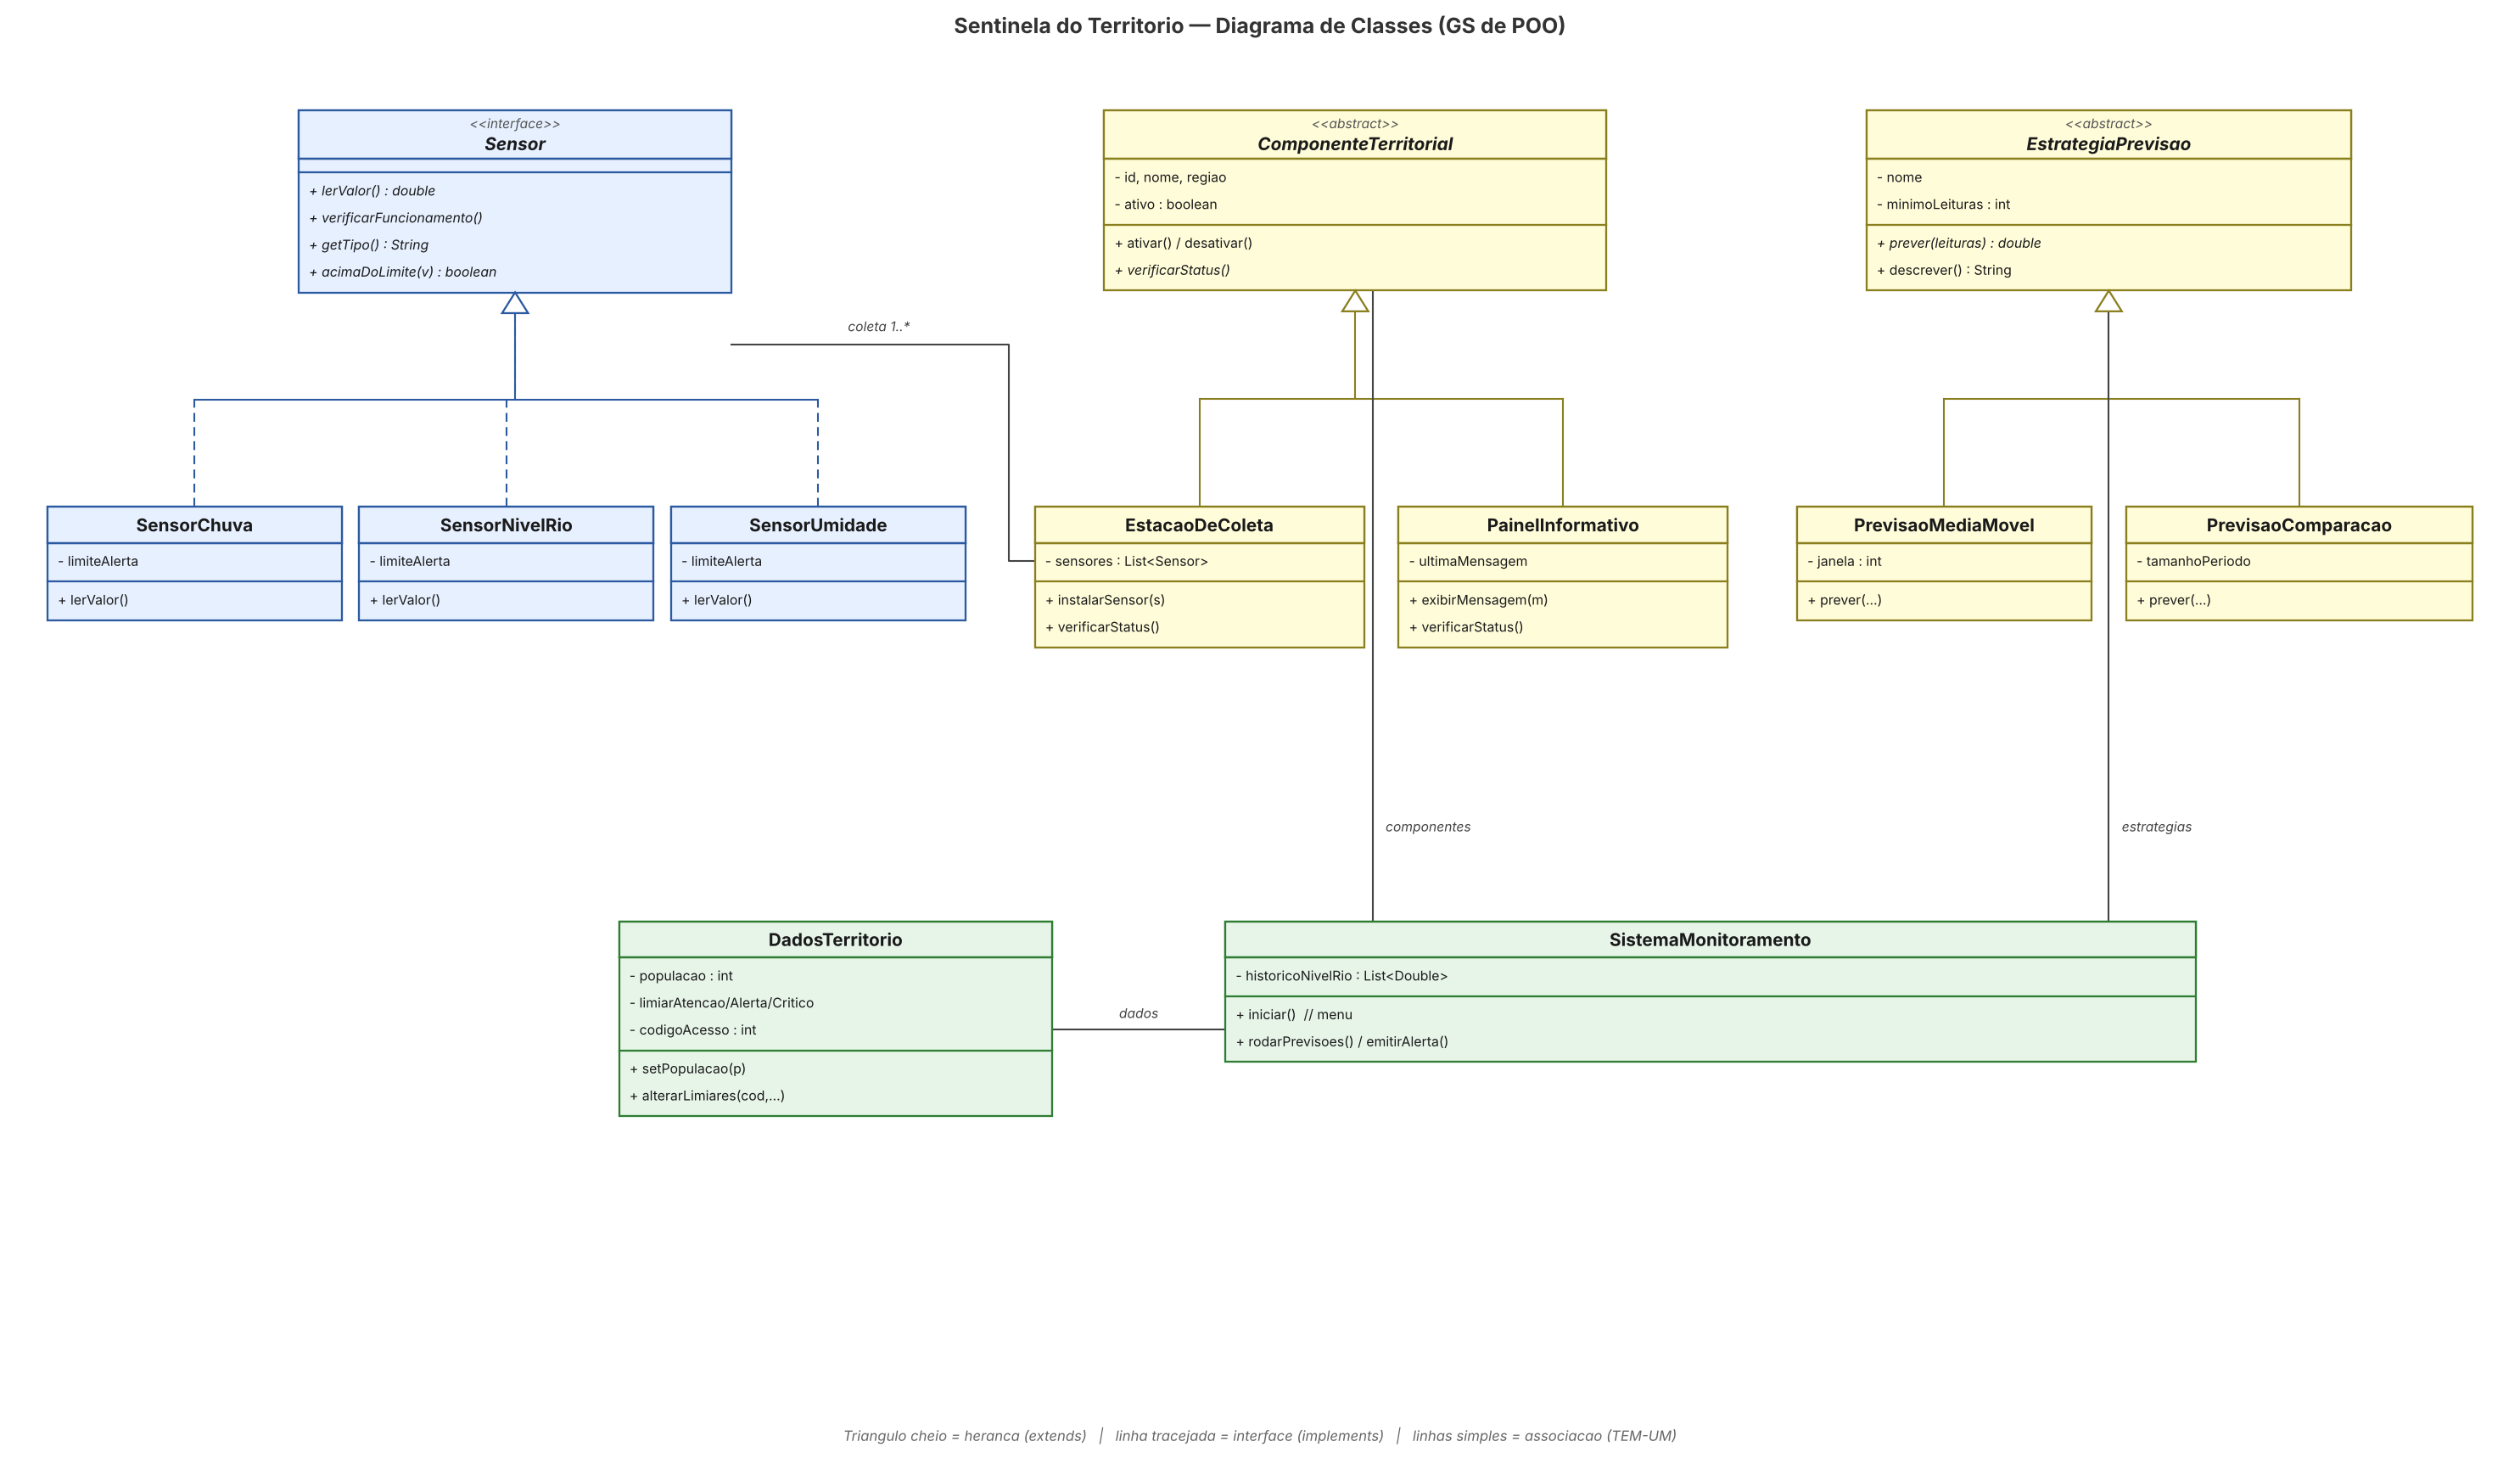
\includegraphics[width=\linewidth]{diagrama_sentinela_gs}
\\[2pt]
{\footnotesize Fonte: elaborado pelos autores (2026).}
\end{figure}

\subsection{Sistema de monitoramento e alertas}
O programa guarda o histórico do nível do rio em um \texttt{ArrayList} e oferece um menu com opções para verificar sensores, rodar previsões, gerenciar os dados do território, simular novas leituras, exibir o status completo e executar uma simulação de 24 horas. O motor de alertas compara a previsão com os limiares do território e classifica a severidade em \texttt{ATENÇÃO}, \texttt{ALERTA} ou \texttt{CRÍTICO}, informando sempre a fonte da previsão, o valor previsto e o limite estourado.

\section{Resultados}

A simulação de 24 horas evidencia o comportamento esperado do sistema: à medida que o nível do rio sobe ao longo do dia, os alertas escalam de \texttt{normal} para \texttt{ATENÇÃO}, depois \texttt{ALERTA} e, por fim, \texttt{CRÍTICO}. Nos testes, a previsão por média móvel acompanhou a tendência de subida, e os alertas foram emitidos com antecedência em relação ao momento em que o limiar crítico foi atingido. As validações de encapsulamento também foram verificadas: tentativas de definir população negativa e de alterar limiares sem o código correto foram rejeitadas, mantendo a integridade dos dados.

\section{Reflexão crítica}

\textbf{Quando o sistema deve se calar?} Com poucas leituras, uma previsão vira chute. Por isso cada estratégia declara um mínimo de leituras e, abaixo desse mínimo, recusa-se a prever. A previsão por comparação, que exige dois períodos completos, permanece em silêncio enquanto não houver dados suficientes, em vez de emitir um número sem lastro — afinal, prever errado mina a confiança no alerta tanto quanto não prever.

\textbf{O que os dados não representam?} Um único sensor de nível por região diz pouco sobre um ponto específico: a média do rio pode estar dentro do limite enquanto uma rua baixa já alaga. As leituras simuladas não capturam bueiros entupidos, obras, maré ou a vulnerabilidade social de cada quarteirão. O número é um indício, não a realidade completa do território.

\textbf{Por que o alerta apoia a decisão, em vez de decidir pela pessoa?} Porque evacuar envolve custo, risco e contexto local que o sistema não enxerga. O Sentinela entrega antecedência e justificativa e deixa a autoridade humana ponderar e agir. Automatizar a leitura é útil; automatizar a decisão de retirar pessoas de casa seria irresponsável.

\section{Considerações finais}

O projeto demonstrou, de forma integrada, os conceitos de classe abstrata, interface, encapsulamento, herança e polimorfismo aplicados a um problema real de monitoramento territorial. Mais do que exercitar a sintaxe da linguagem, o trabalho reforçou uma postura de projeto: proteger dados sensíveis, reconhecer os limites do que os dados representam e construir um sistema que apoia a decisão humana. Como evolução, a equipe considera incorporar dados reais de fontes públicas e ampliar as estratégias de previsão.

\begin{thebibliography}{9}
\bibitem{deitel} DEITEL, Paul; DEITEL, Harvey. \textit{Java: como programar}. 10. ed. São Paulo: Pearson, 2017.
\bibitem{oracle} ORACLE. \textit{The Java Tutorials: Object-Oriented Programming Concepts}. Disponível em: https://docs.oracle.com/javase/tutorial/java/concepts/. Acesso em: 6 nov. 2026.
\bibitem{anjos} ANJOS, Ygor Moraes Martins dos. \textit{Global Solution 2/2026 -- POO: Territory Predictive Insights (CitizenTech)}. São Paulo: FIAP, 2026.
\end{thebibliography}

\end{document}
